\documentclass[dvipdfmx]{report} % 文章の形式を設定
\usepackage[margin=2.5cm]{geometry} % 書式の空白を設定
\usepackage[utf8]{inputenc} % 文字コードをUTF-8に設定
\usepackage{hyperref} % 目次にリンクを付けるため
\usepackage{lipsum} % ダミーテキスト用
\usepackage{tcolorbox} % 枠を利用するため
\usepackage{amsmath} % 数式の記述を行うため
\usepackage{bm} % ベクトルを太字で表示するため
\usepackage{graphicx} % 画像を表示するため
\usepackage{float} % 画像正しい位置で表示するため
\usepackage{tensor} % テンソルを記載するため
\usepackage{multicol} % 複数段落を作成するため
\usepackage{tikz} % 図を作成するため
\usepackage{enumerate} % リストを作成するため
\usepackage{amssymb} % 特殊文字を表示するため
\usepackage{color} % 文字の色を指定するため


\title{降着円盤の像}
\author{大豆生田 幹}
\date{}

\begin{document}

\maketitle % タイトルの作成
\tableofcontents % 目次の作成
\fontsize{11pt}{11pt}\selectfont % 文字サイズの指定


% =================================
% =================================
% =================================
% =================================
% =================================
% 光の条件
% =================================
% =================================
% =================================
% =================================
% =================================
\chapter{null条件}
超大質量天体は降着円盤と呼ばれる、ガスなどの物質で構成された円盤を持つことが多い。降着円盤は中心天体を高速で公転しており、摩擦の影響で電磁波を放っている。
今回は、重力中心から一定距離に幾何学的に薄い降着円盤を設定し、それがどのように観測されるのかを計算する。

この計算をするためには、時空上で光の軌道が満たす方程式と、光の軌道が満たす条件を考慮する必要がある。ここではその条件を導出する。
\section{クラインゴルドン方程式}
クラインゴルドン場を$\phi(x, t)$とすると、クラインゴルドン方程式は以下のように書ける。
\[
	\left( \square+m^2 \right) \phi(x, t) = 0
\]
($c=1, \hbar=1$の単位系を用いた。)この式を計量$g_{ij}$で表される一般の時空に拡張し、$m=0$の波を考えると、式は以下のように変形できる。
\begin{equation}
\begin{split}
	0 = g^{ij}\nabla_{i}\nabla_{j}\phi(x)
\end{split}
\end{equation}
振動数が非常に大きい波を考えると、波は以下のように書ける。
\begin{equation}
\begin{split}
	\phi(x) = C(x)\exp{ \left( \frac{S(x)}{\epsilon}i \right) } \quad \epsilon \ll 1
\end{split}
\end{equation}
以上をまとめると、以下の式を導くことができる。
\begin{equation*}
\begin{split}
	0 = g^{jk}(x)\nabla_{j}\nabla_{k}
		\left[ C(x)\exp{ \left( \frac{S(x)}{\epsilon}i \right) } \right]
\end{split}
\end{equation*}

\section{null条件の導出}
上記で求めた式を少しづつ計算していく
\begin{equation*}
\begin{split}
	\nabla_k \left[ C(x)\exp{ \left( \frac{S(x)}{\epsilon}i \right) } \right] &= 
		\left[
			( \nabla_k C(x) )
			+ \left( \frac{C(x)}{\epsilon}i \right) (\nabla_k S(x)) 
		\right] \exp \left( \frac{S(x)}{\epsilon} i \right)\\
	\nabla_j \nabla_k \left[ C(x)\exp{ \left( \frac{S(x)}{\epsilon}i \right) } \right] &= 
		[
			\nabla_j \nabla_k C(x)
			+ \frac{2}{\epsilon}i (\nabla_j C(x))(\nabla_k S(x))\\
		& \quad
			+ \frac{C(x)}{\epsilon}i (\nabla_j \nabla_k S(x))
			- \frac{C(x)}{\epsilon ^ 2}i (\nabla_j S(x))(\nabla_k S(x))
		] \exp \left( \frac{S(x)}{\epsilon} i \right)\\
	g^{jk}(x) \nabla_j \nabla_k \left[ C(x)\exp{ \left( \frac{S(x)}{\epsilon}i \right) } \right]
		&=
			g^{jk}(x) \nabla_j \nabla_k C(x) \exp \left( \frac{S(x)}{\epsilon} i \right) \\
		&\quad
			+ \left[
				2(\nabla_j C(x))(\nabla_k S(x)) + C(x) (\nabla_j \nabla_k S(x))
			\right]
			\frac{ g^{jk}(x) }{\epsilon}i \exp \left( \frac{S(x)}{\epsilon} i \right)\\
		&\quad
			- C(x) (\nabla_j S(x))(\nabla_k S(x)) \frac{ g^{jk}(x) }{\epsilon ^ 2}i 				\exp \left( \frac{S(x)}{\epsilon} i \right)
\end{split}
\end{equation*}
ここで書いた項はすべてゼロになるので
\begin{equation*}
\begin{split}
\left\{ \,
\begin{aligned}
	 O(0) &: g^{jk}(x) \nabla_j \nabla_k C(x) = 0\\
	 O(\epsilon^{-1}) &:
	 	2g^{jk}(x)(\nabla_j C(x))(\nabla_k S(x))
		+ g^{jk}(x)C(x) (\nabla_j \nabla_k S(x)) = 0\\
   	O(\epsilon^{-2}) &:
		g^{jk}(x) (\nabla_j S(x))(\nabla_k S(x)) = 0\\
\end{aligned}
\right.
\end{split}
\end{equation*}
光の波数ベクトル$\bold{k}$に対して以下の関係式が成り立つと仮定する。
\[ \nabla^i S = k^i \]
すると、$O(\epsilon^{-2})$式は以下のように書き換えられる。
\[0 = k^i k_i\]
これが光の軌道が満たす条件であり、以降はnull条件と呼ぶ。

% =================================
% =================================
% =================================
% =================================
% =================================
% シュバルツシルト解
% =================================
% =================================
% =================================
% =================================
% =================================
\chapter{シュバルツシルト解}
一般相対論による強い重力の効果は、シュバルツシルト時空と呼ばれる静的で真空球対称のブラックホール解を典型的な例として理解できる。まずはこの時空における降着円盤の像を計算しよう。\\
まず、シュバルツシルト時空の線素は以下のように書くことができる。
\[
ds^2 =
		-\left( 1 - \frac{2M}{r} \right)dt^2
		+ \left( 1 - \frac{2M}{r} \right)^{-1}dr^2
		+ r^2( d\theta^2 + \sin^2\theta d\phi^2 )
\]
天体が作る重力場は漸近的に平坦であると考えられるが、この解は$r \rightarrow \infty$でその条件を満たしている。

% =================================
% 光の軌道を表す微分方程式の導出
% =================================
\section{光の軌道が満たす微分方程式の導出}
力を加えない限り曲がった時空上の物質は距離が停留点をとるような軌道を描くことが知られており、このような軌道を測地線と呼ぶ。ここではシュバルツシルト時空における光の軌道を表す微分方程式を導出する。\\
距離を$S$、光の軌道を表すパラメータであり、波数ベクトルに対して
\[
	k^i = \frac{d x^i}{d \lambda}
\]
を満たすようなパラメータをアフィンパラメータと呼び、$\lambda$と書くと、距離は以下のように書ける。
\begin{equation*}
\begin{split}
	S &= \int \mathcal{L} d\lambda \\
	&= \int \frac{1}{2} \left(
		-\left( 1 - \frac{2M}{r} \right)\dot{t}^2
		+ \left( 1 - \frac{2M}{r} \right)^{-1}\dot{r}^2
		+ r^2( d\theta^2 + \sin^2\theta \dot{\phi}^2 )
	\right) d\lambda
\end{split}
\end{equation*}
シュバルツシルト時空は球対称であり、光は特定の赤道面に囚われた軌道をとることになるので$\theta = \frac{\pi}{2}$の面に注目することにすれば、以下のように書き換えることができる。
\[
S = 	\int \frac{1}{2} \left(
		-\left( 1 - \frac{2M}{r} \right)\dot{t}^2
		+ \left( 1 - \frac{2M}{r} \right)^{-1}\dot{r}^2
		+ r^2\dot{\phi}^2 )
	\right) d\lambda
\]
この距離が停留点を取るので、オイラーラグランジュ方程式より
\begin{equation*}
\begin{split}
	0 &
		= - \frac{d}{d\lambda}\left( \frac{d\mathcal{L}}{d\dot{t}} \right)
		= \left( 1 - \frac{2M}{r} \right) \dot{t}\\
	\text{ \textcolor{red}{エネルギー保存則} } &\therefore  E = \left( 1 - \frac{2M}{r} \right) \dot{t}\\
	0 &
		= \frac{d}{d\lambda}\left( \frac{d\mathcal{L}}{d\dot{\phi}} \right)
		= r^2 \dot{\phi}\\
	\text{ \textcolor{red}{角運動量保存則} } &\therefore  L = r^2  \dot{\phi}\\
\end{split}
\end{equation*}
また、null条件 $0=k^ik_i$より
\begin{tcolorbox}[title=シュバルツシルト時空における光の方程式]
\begin{eqnarray*}
	0 &= -\left( 1 - \frac{2M}{r} \right)\dot{t}^2
		+ \left( 1 - \frac{2M}{r} \right)^{-1}\dot{r}^2
		+ r^2\dot{\phi}^2\\
	&\therefore
		\left( \frac{E}{L} \right)^2 =
			\frac{1}{r^2} \left( \frac{dr}{d\phi} \right)^2
			+ \frac{1}{r^2} \left( 1 - \frac{2M}{r} \right)
\end{eqnarray*}
\end{tcolorbox}
後の計算のために、衝突係数$b = \frac{L}{E}$、有効ポテンシャル$\mathrm{V_{eff}}$、$u=\frac{1}{r}$を導入して式を書き換えておく。
\begin{equation*}
\begin{split}
	G(u) 	&= \left( \frac{du}{d\phi} \right)^2\\ 
	\left( \frac{1}{b} \right)^2 &=
			u^2 G(u) + \mathrm{V_{eff}(u)}\\
\end{split}
\end{equation*}

% =================================
% 有効ポテンシャルの解析
% =================================
\section{有効ポテンシャルの解析}
有効ポテンシャルは以下のような形になっている。
\begin{figure}[H]
    \centering
    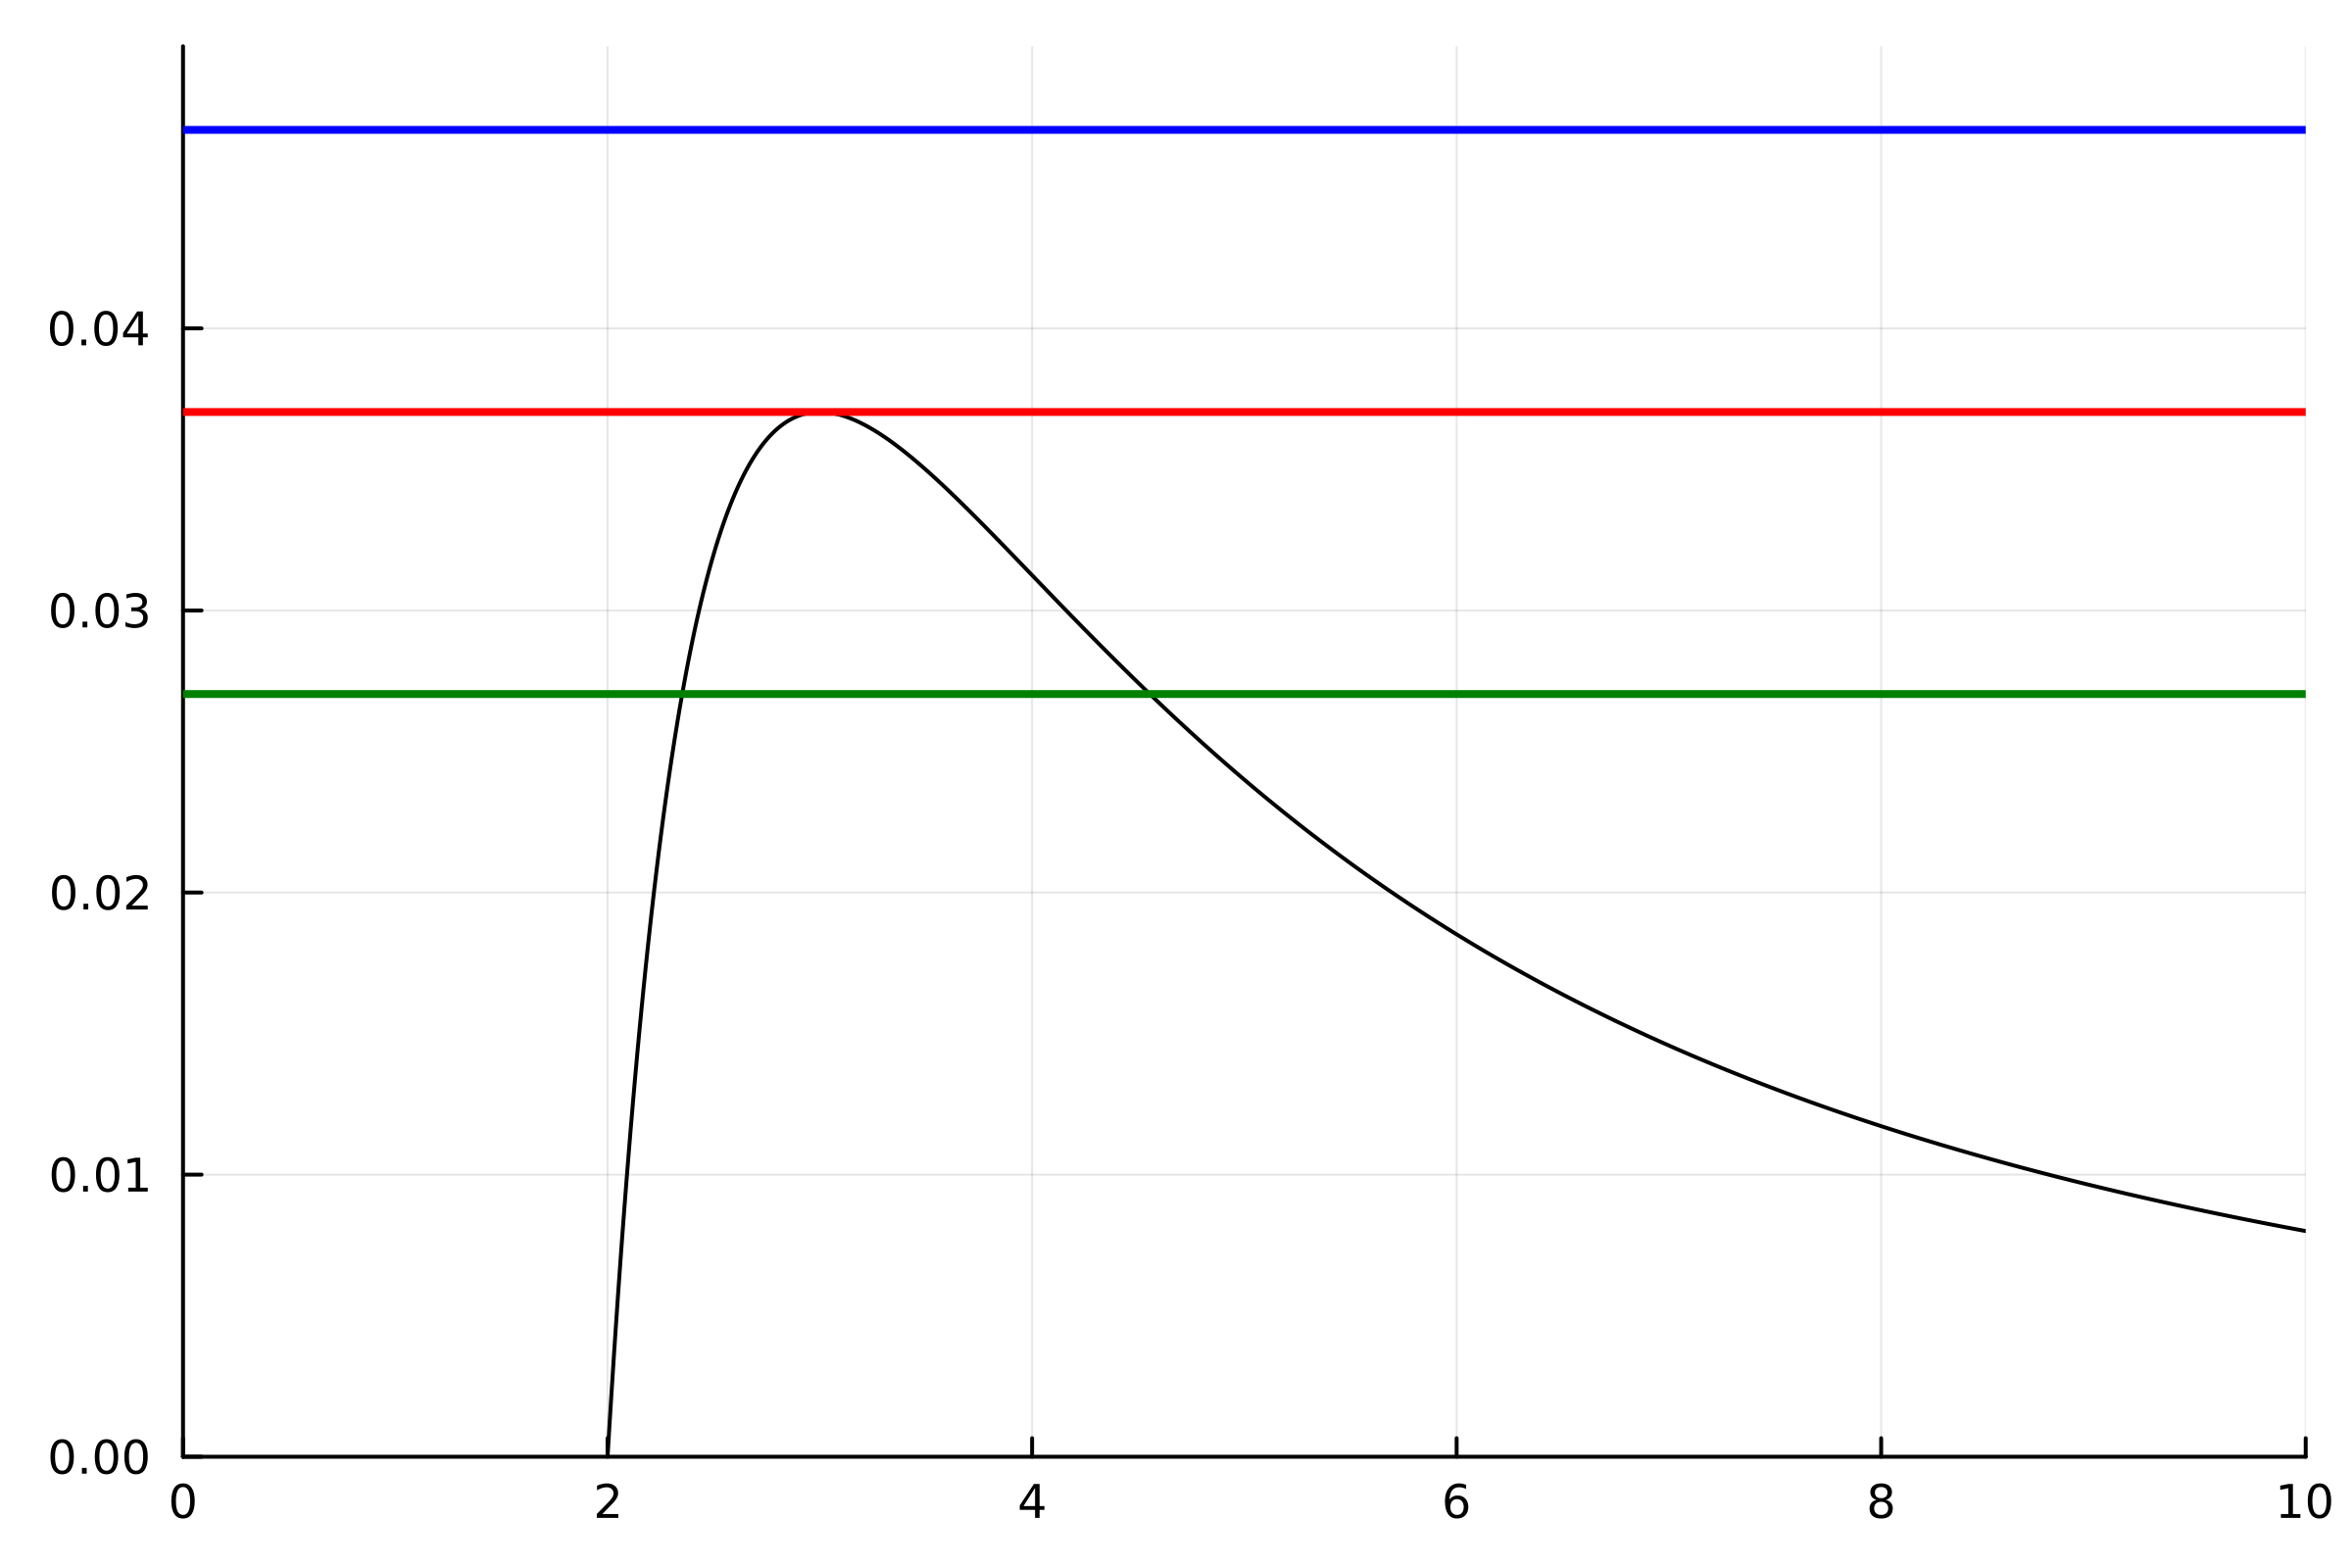
\includegraphics[width=0.5\columnwidth]{./images/schwa/v-eff.png}
    \caption{有効ポテンシャル(縦軸$V_{\mathrm{eff}}$ - 横軸$r/M$)}
    \label{}
\end{figure}
これを解析し、ある有効ポテンシャルをもつ光がどのような軌道をとるか考える。
\begin{equation*}
\begin{split}
	V_{\mathrm{eff}} &= \frac{1}{r^2} \left( 1 - \frac{2M}{r} \right) \\
	V_{\mathrm{eff}}' &= \frac{2M}{r^4} \left( 3 - \frac{r}{M} \right) \\
\end{split}
\end{equation*}
この式からわかることをまとめると、以下のようになる。
\begin{enumerate}[(1)\,]
\item{有効ポテンシャルが\textcolor{blue}{青線}の大きさを持つ光の軌道($1/27 < V_{\mathrm{eff}}$)}\\
この光は重力中心へ落下、もしくは無限遠まで飛んでゆく軌道とる。
\item{有効ポテンシャルが\textcolor{red}{赤線}の大きさを持つ光の軌道($1/27 = V_{\mathrm{eff}}$)}\\
この光は不安定ではあるが、円軌道をとる。
\item{有効ポテンシャルが\textcolor{green}{緑線}の大きさを持つ光の軌道($1/27 > V_{\mathrm{eff}}$)}\\
この光はあるところまで重力中心まで近づき、散乱されて無限遠に飛んでゆく軌道をとる。
\end{enumerate}


% =================================
% 光の軌道を表す微分方程式の導出
% =================================
\section{有効ポテンシャルの解析}

% =================================
% =================================
% =================================
% =================================
% =================================
% ブハダール解
% =================================
% =================================
% =================================
% =================================
% =================================
\chapter{ブハダール解}
続いて、曲率特異点を持たず、ホライズンも存在しないような自然な時空であるブハダール時空に着目し、降着円盤の見え方を考える。ブハダール時空の線素は以下のように書くことができる。
\begin{equation*}
\begin{split}
	ds^2 &=
		- \frac{(1 - f(r))^2}{(1 + f(r))^2} dt^2
		+ (1 + f(r))^4 dr^2
		+ r^2(1 + f(r))^4 d\theta^2
		+ r^2 (1 + f(r))^4 \sin ^2 \theta d\phi^2 \\
	f(r) &= \frac{a}{2\sqrt{1 + k r^2}} 
\end{split}
\end{equation*}
この解も$r \rightarrow \infty$で平坦な時空に漸近する。

% =================================
% 光の軌道を表す微分方程式の導出
% =================================
\section{光の軌道が満たす微分方程式の導出}
ブハダール時空は球対称であり、光は特定の赤道面に囚われた軌道をとることになるので$\theta = \frac{\pi}{2}$の面に注目することにすれば、距離は以下のように書ける。
\begin{equation*}
\begin{split}
	S  &= \int \mathcal{L} d\tau \\
	&=  \int \left(
			- \frac{(1 - f(r))^2}{(1 + f(r))^2} \dot{t}^2
			+ (1 + f(r))^4 \dot{r}^2
			+ r^2(1 + f(r))^4 \dot{\phi}^2
		\right) d\tau
\end{split}
\end{equation*}
この距離が停留点を取るので、オイラーラグランジュ方程式より
\begin{equation*}
\begin{split}
	0 &
		= - \frac{1}{2}\left( \frac{d\mathcal{L}}{d\dot{t}} \right)
		= \frac{ (1 - f(r))^2 }{(1 + f(r))^2} \dot{t}\\
	&\therefore  E = \frac{(1 - f(r))^2 }{(1 + f(r))^2} \dot{t}\\
	0 &
		= \frac{1}{2}\left( \frac{d\mathcal{L}}{d\dot{\phi}} \right)
		= r^2 (1 + f(r))^4  \dot{\phi}\\
	&\therefore  L = r^2 (1 + f(r))^4  \dot{\phi}\\
\end{split}
\end{equation*}
また、null条件 $0=k^ik_i$より
\begin{equation*}
\begin{split}
	0 &=
		- \frac{(1 - f(r))^2}{(1 + f(r))^2} \dot{t}^2
		+ (1 + f(r))^4 \dot{r}^2
		+ r^2(1 + f(r))^4 \dot{\phi}^2\\
	& \therefore 
		\left( \frac{E}{L} \right)^2 =
			\frac{(1 - f(r))^2}{r^4 (1 + f(r))^6} \left( \frac{dr}{d\phi} \right)^2
			+ \frac{(1 - f(r))^2}{r^2 (1 + f(r))^6}
\end{split}
\end{equation*}
これが、ブハダール時空における光の軌道が満たすべき式である。

後の計算のために、衝突係数$b = \frac{L}{E}$、有効ポテンシャル$\mathrm{V_{eff}}$、$u=\frac{1}{r}$を導入して式を書き換えておく。
\begin{equation*}
\begin{split}
	G(u) 	&= \left( \frac{du}{d\phi} \right)^2\\ 
	\left( \frac{1}{b} \right)^2 &=
			\frac{u^4 (1-f(u))^2}{(1+f(u))^6} G(u)
			+ \mathrm{V_{eff}(u)}\\
\end{split}
\end{equation*}
有効ポテンシャルは以下のような形になっている。
\begin{figure}[H]
    \centering
    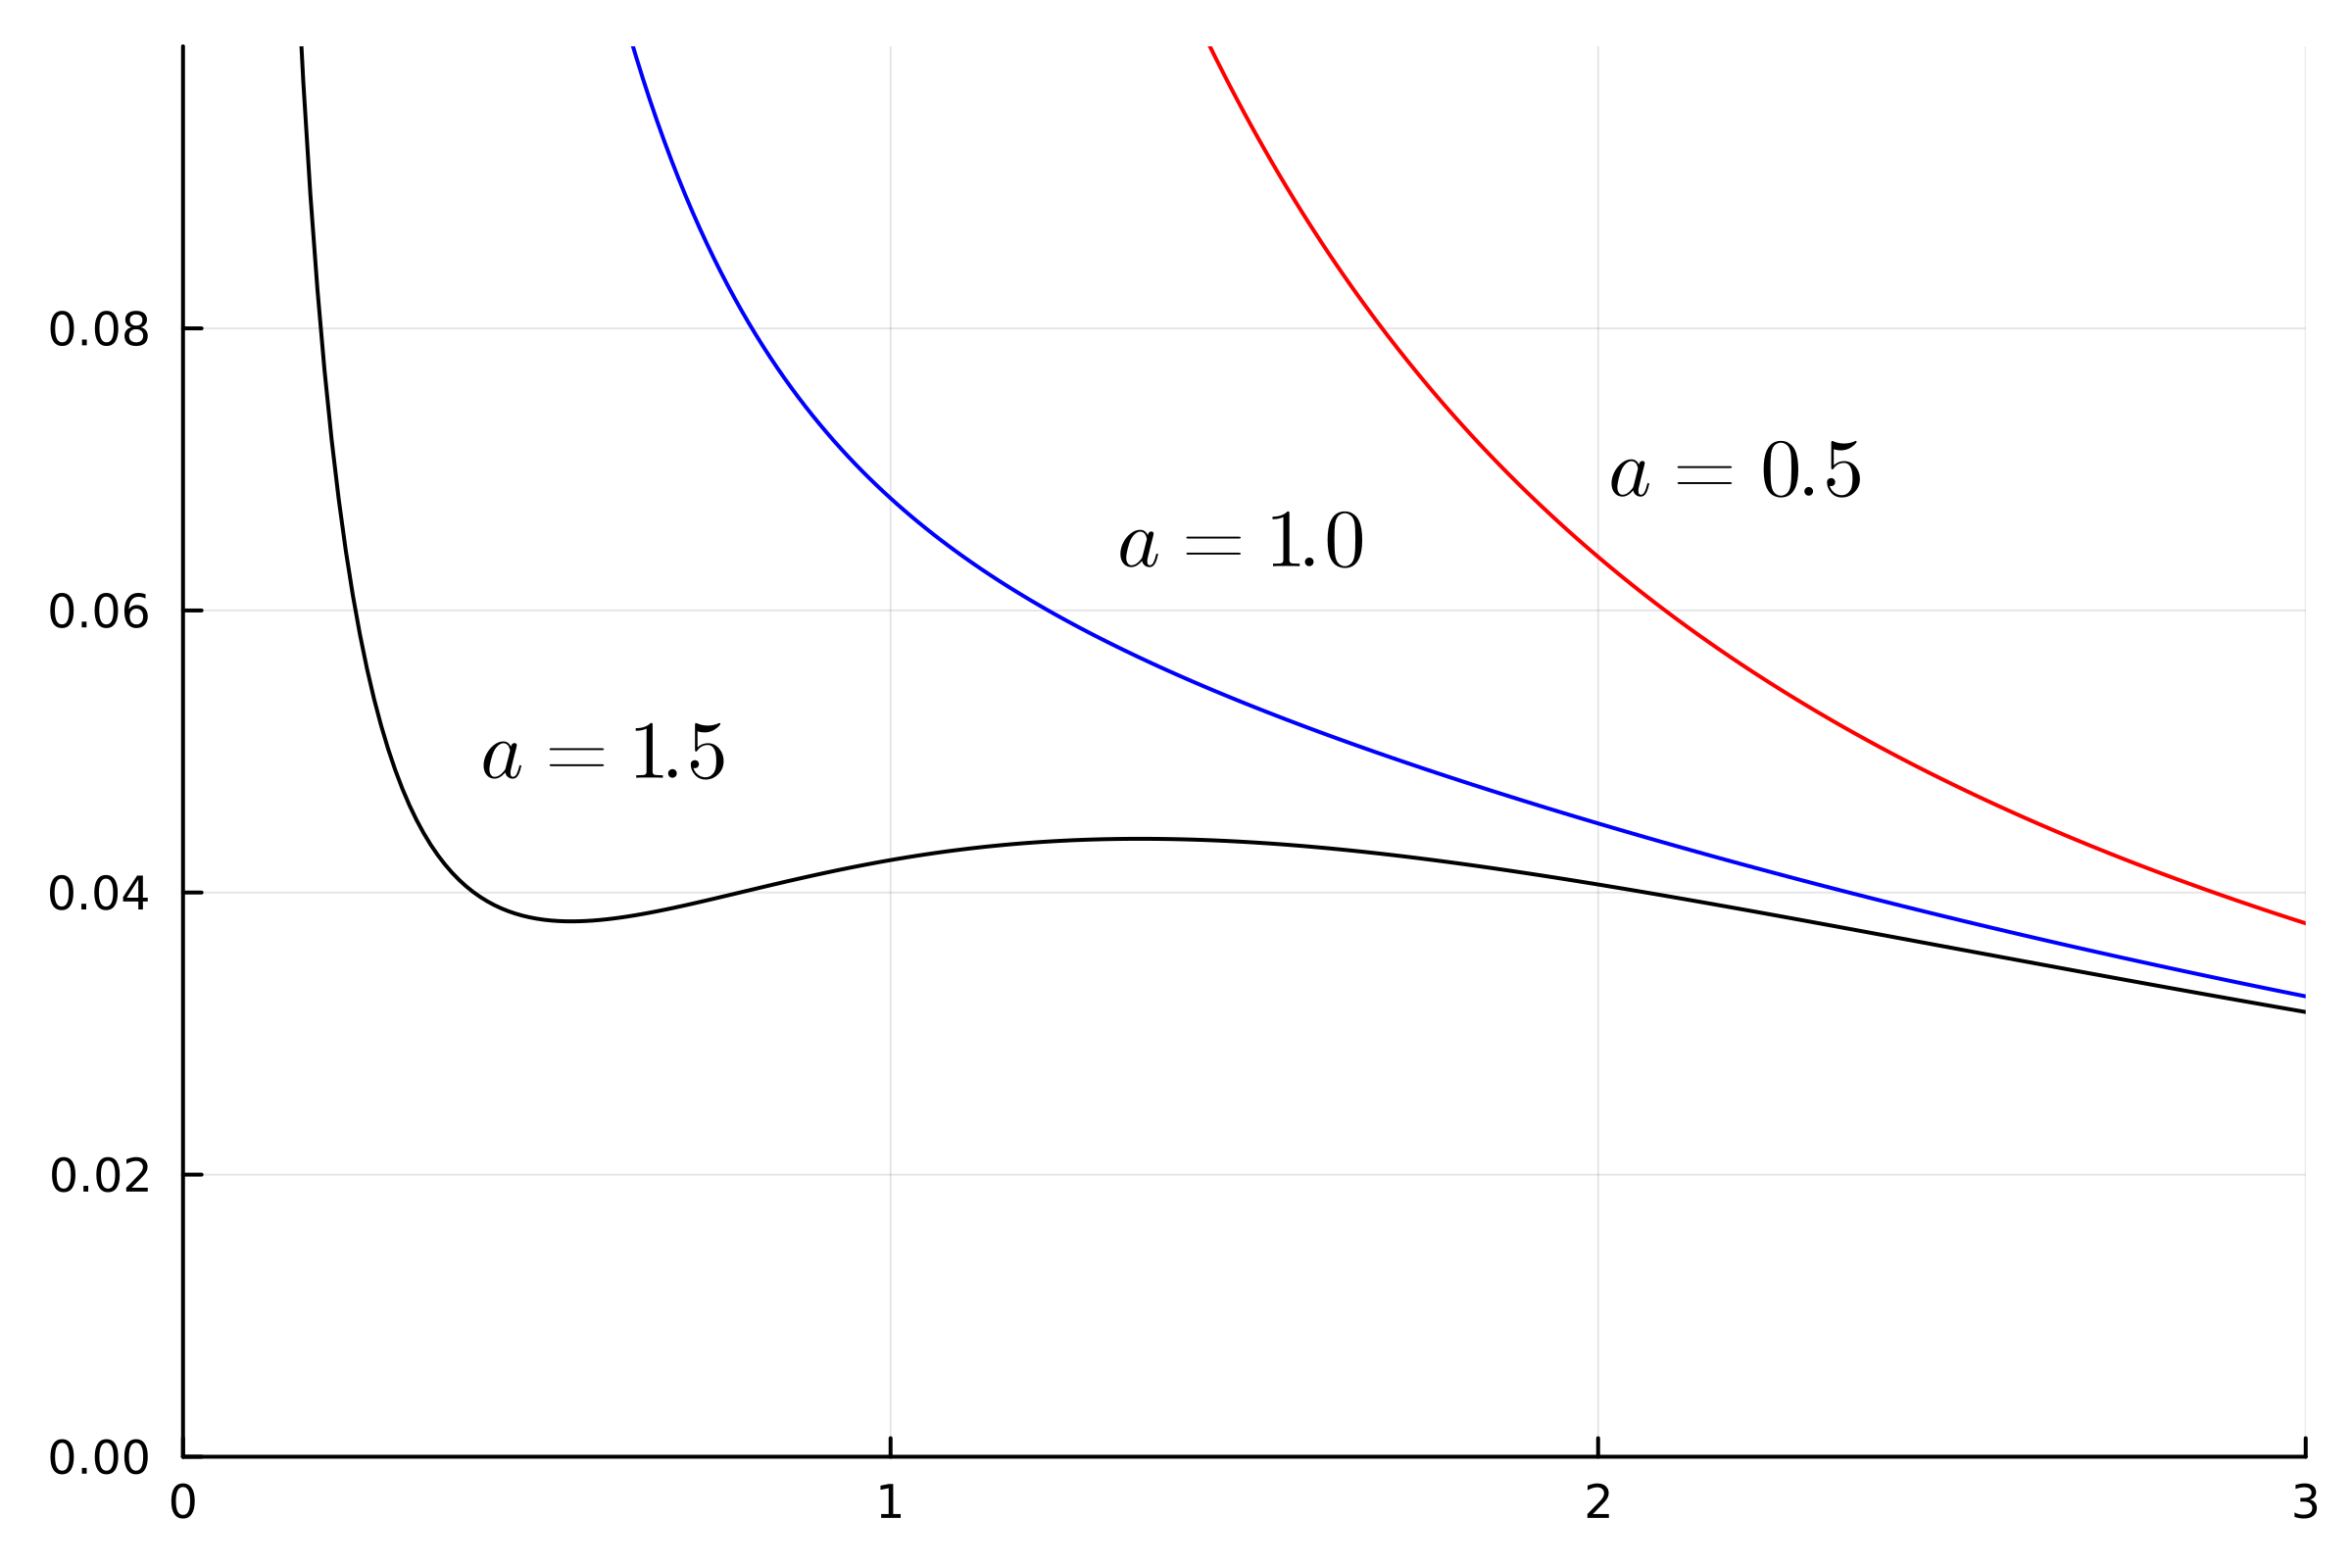
\includegraphics[width=0.5\columnwidth]{./images/buch/v-eff.png}
    \caption{有効ポテンシャル}
    \label{}
\end{figure}

% =================================
% パラメータの制約
% =================================
\section{パラメータの制約}

% =================================
% 光の軌道の解析
% =================================
\section{光の軌道の解析}

\begin{figure}[H]
    \centering
    \begin{minipage}{0.49\textwidth}
        \centering
        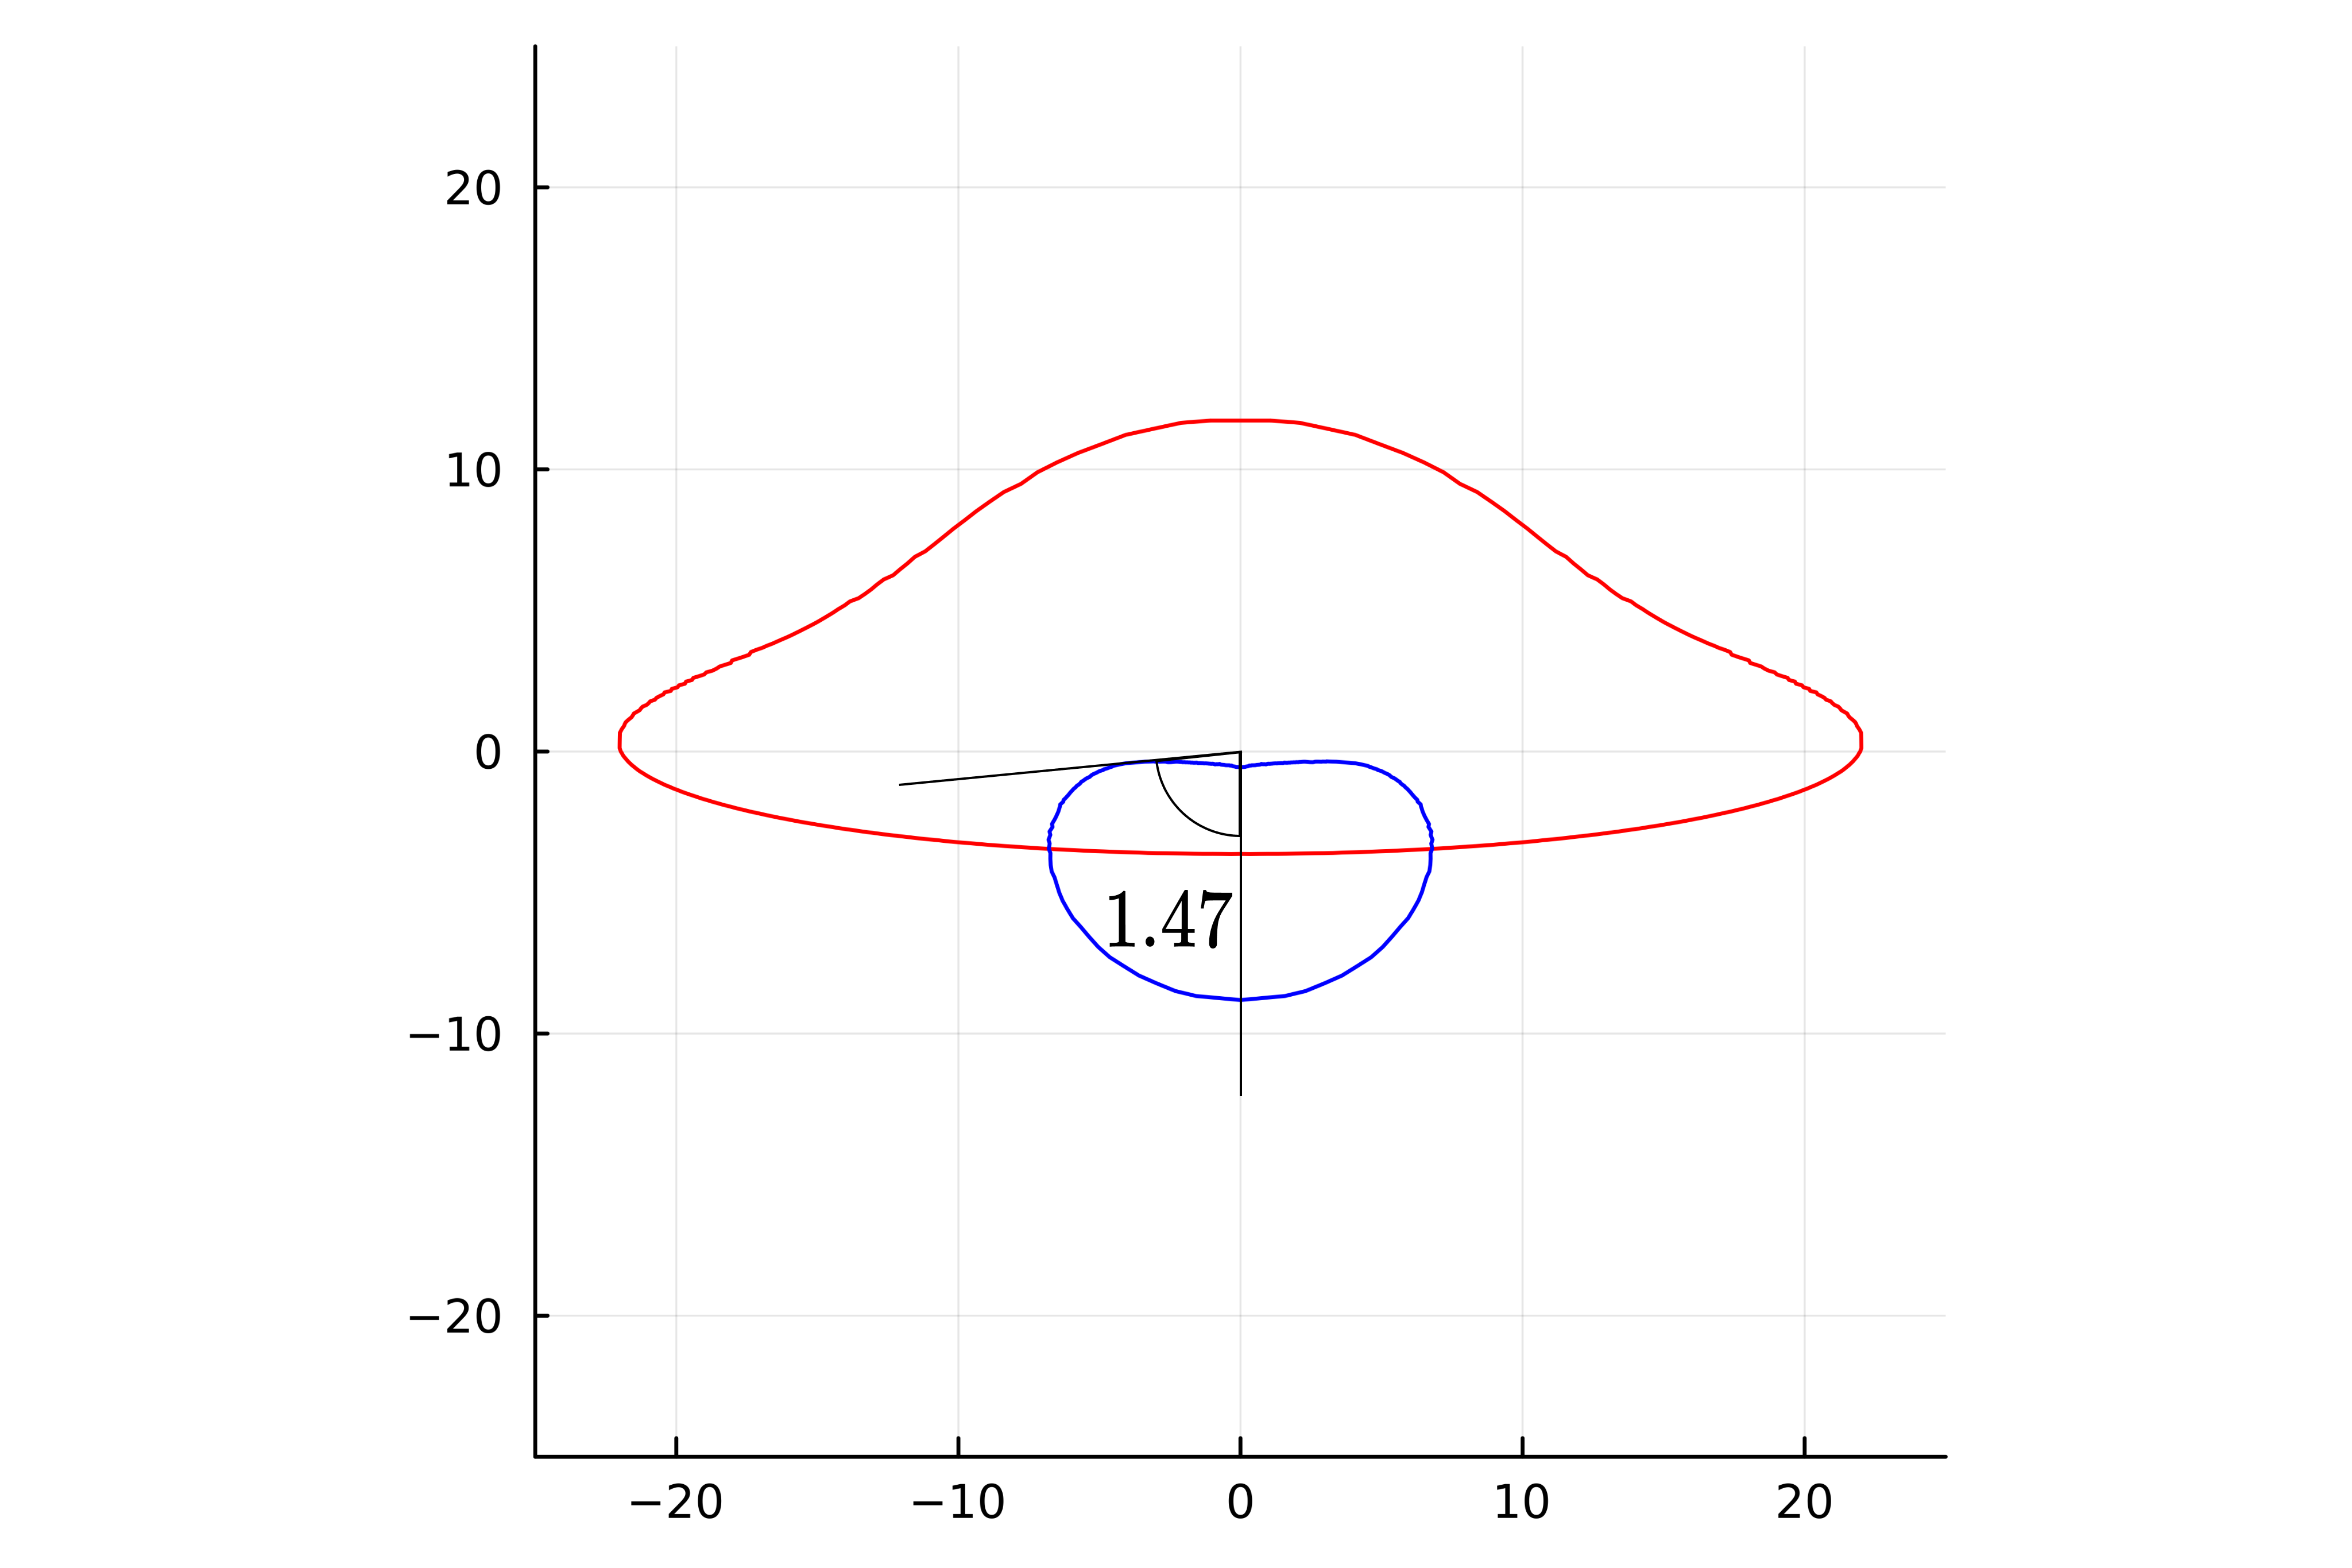
\includegraphics[width=\textwidth]{./images//buch/80/80-0.5.png}
        \caption{$\theta_{0}=80^{o} \quad a=0.5$}
        \label{}
    \end{minipage}
    \begin{minipage}{0.49\textwidth}
        \centering
        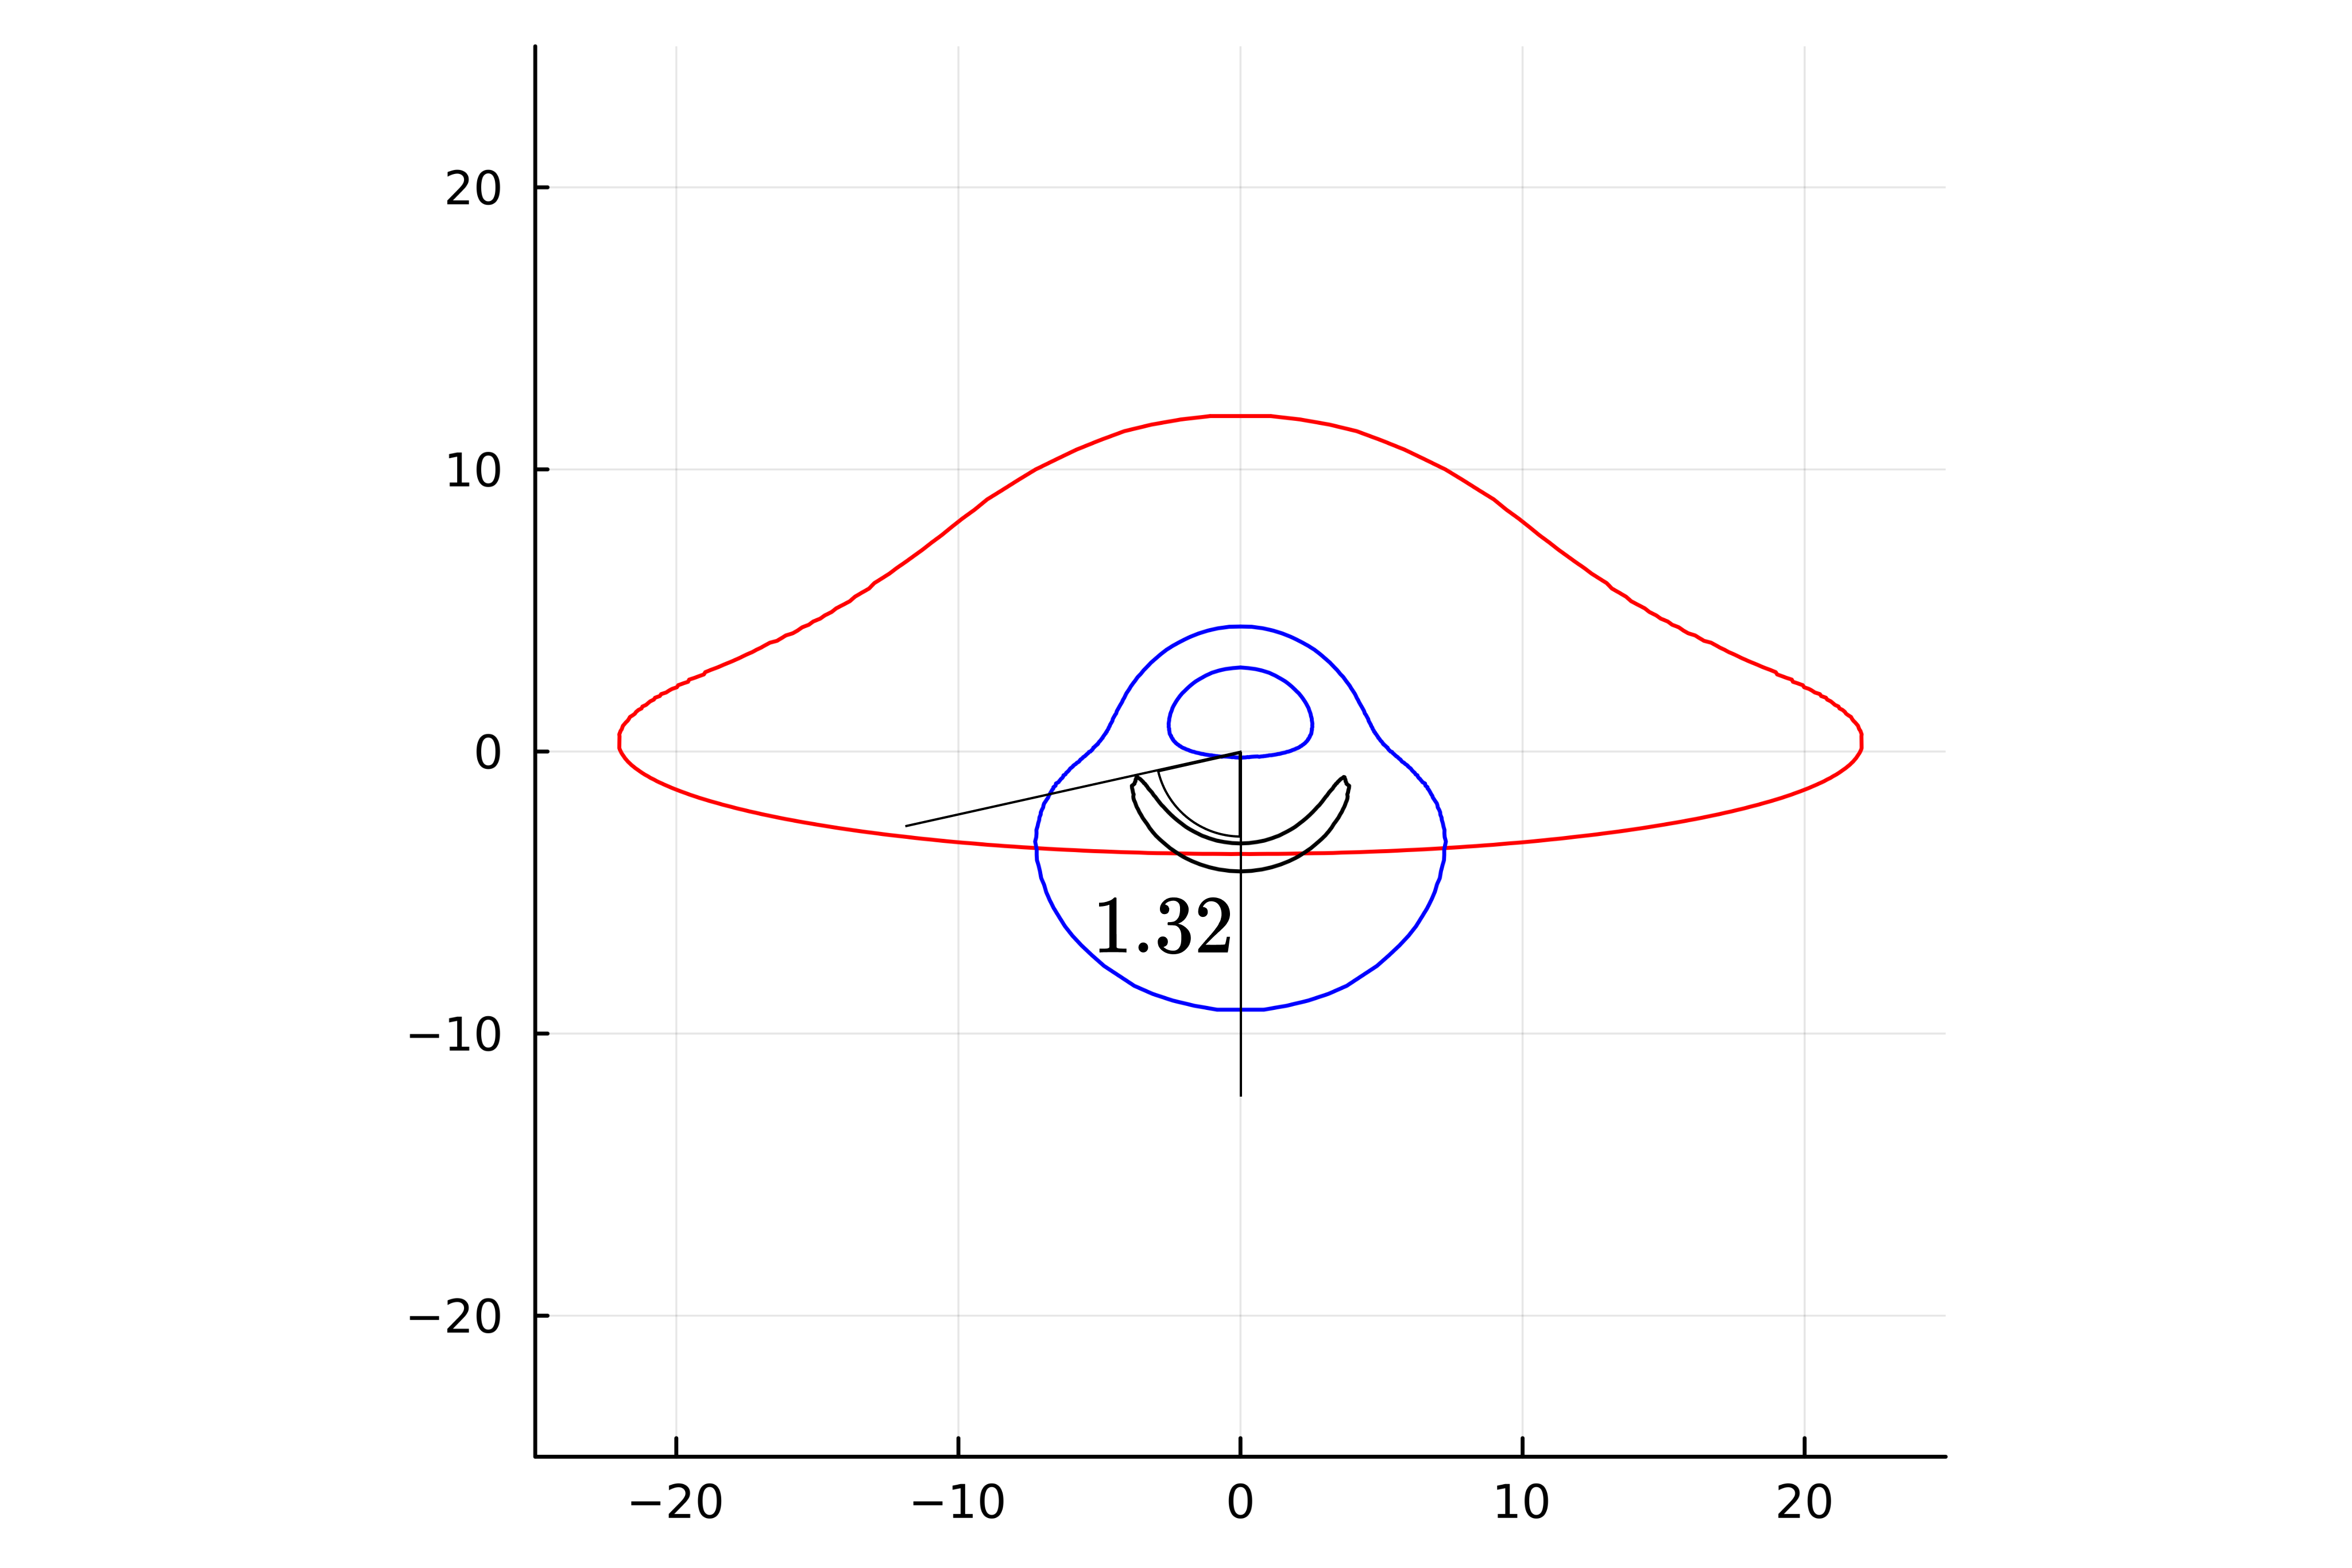
\includegraphics[width=\textwidth]{./images//buch/80/80-1.0.png}
        \caption{$\theta_{0}=80^{o} \quad a=1.0$}
        \label{}
    \end{minipage}
    \begin{minipage}{0.49\textwidth}
        \centering
        \includegraphics[width=\textwidth]{./images//buch/80/80-1.5.png}
        \caption{$\theta_{0}=80^{o} \quad a=1.5$}
        \label{}
    \end{minipage}
\end{figure}




\chapter{コピペ用テキスト}
/////////////////////////////////////////////////////////////////////////\\
/////////////////////////////////////////////////////////////////////////
\textcolor{red}{テスト}

% 方程式
\begin{equation*}
\begin{split}
	\bar{w}_j = \left( \right) \int^{}_{}
\end{split}
\end{equation*}

% ボックス
\begin{tcolorbox}[title=メモ用]
\begin{eqnarray*}
	1 = 0
\end{eqnarray*}
\end{tcolorbox}

% { 付き方程式
\begin{equation}
\left\{ \,
\begin{aligned}
	1 &= 0\\
	1 &= 0\\
\end{aligned}
\right.
\end{equation}

% 行列
\[
\left(
\begin{matrix}
a & b \\
c & d
\end{matrix}
\right)
\]


% 画像
\begin{figure}[H]
    \centering
    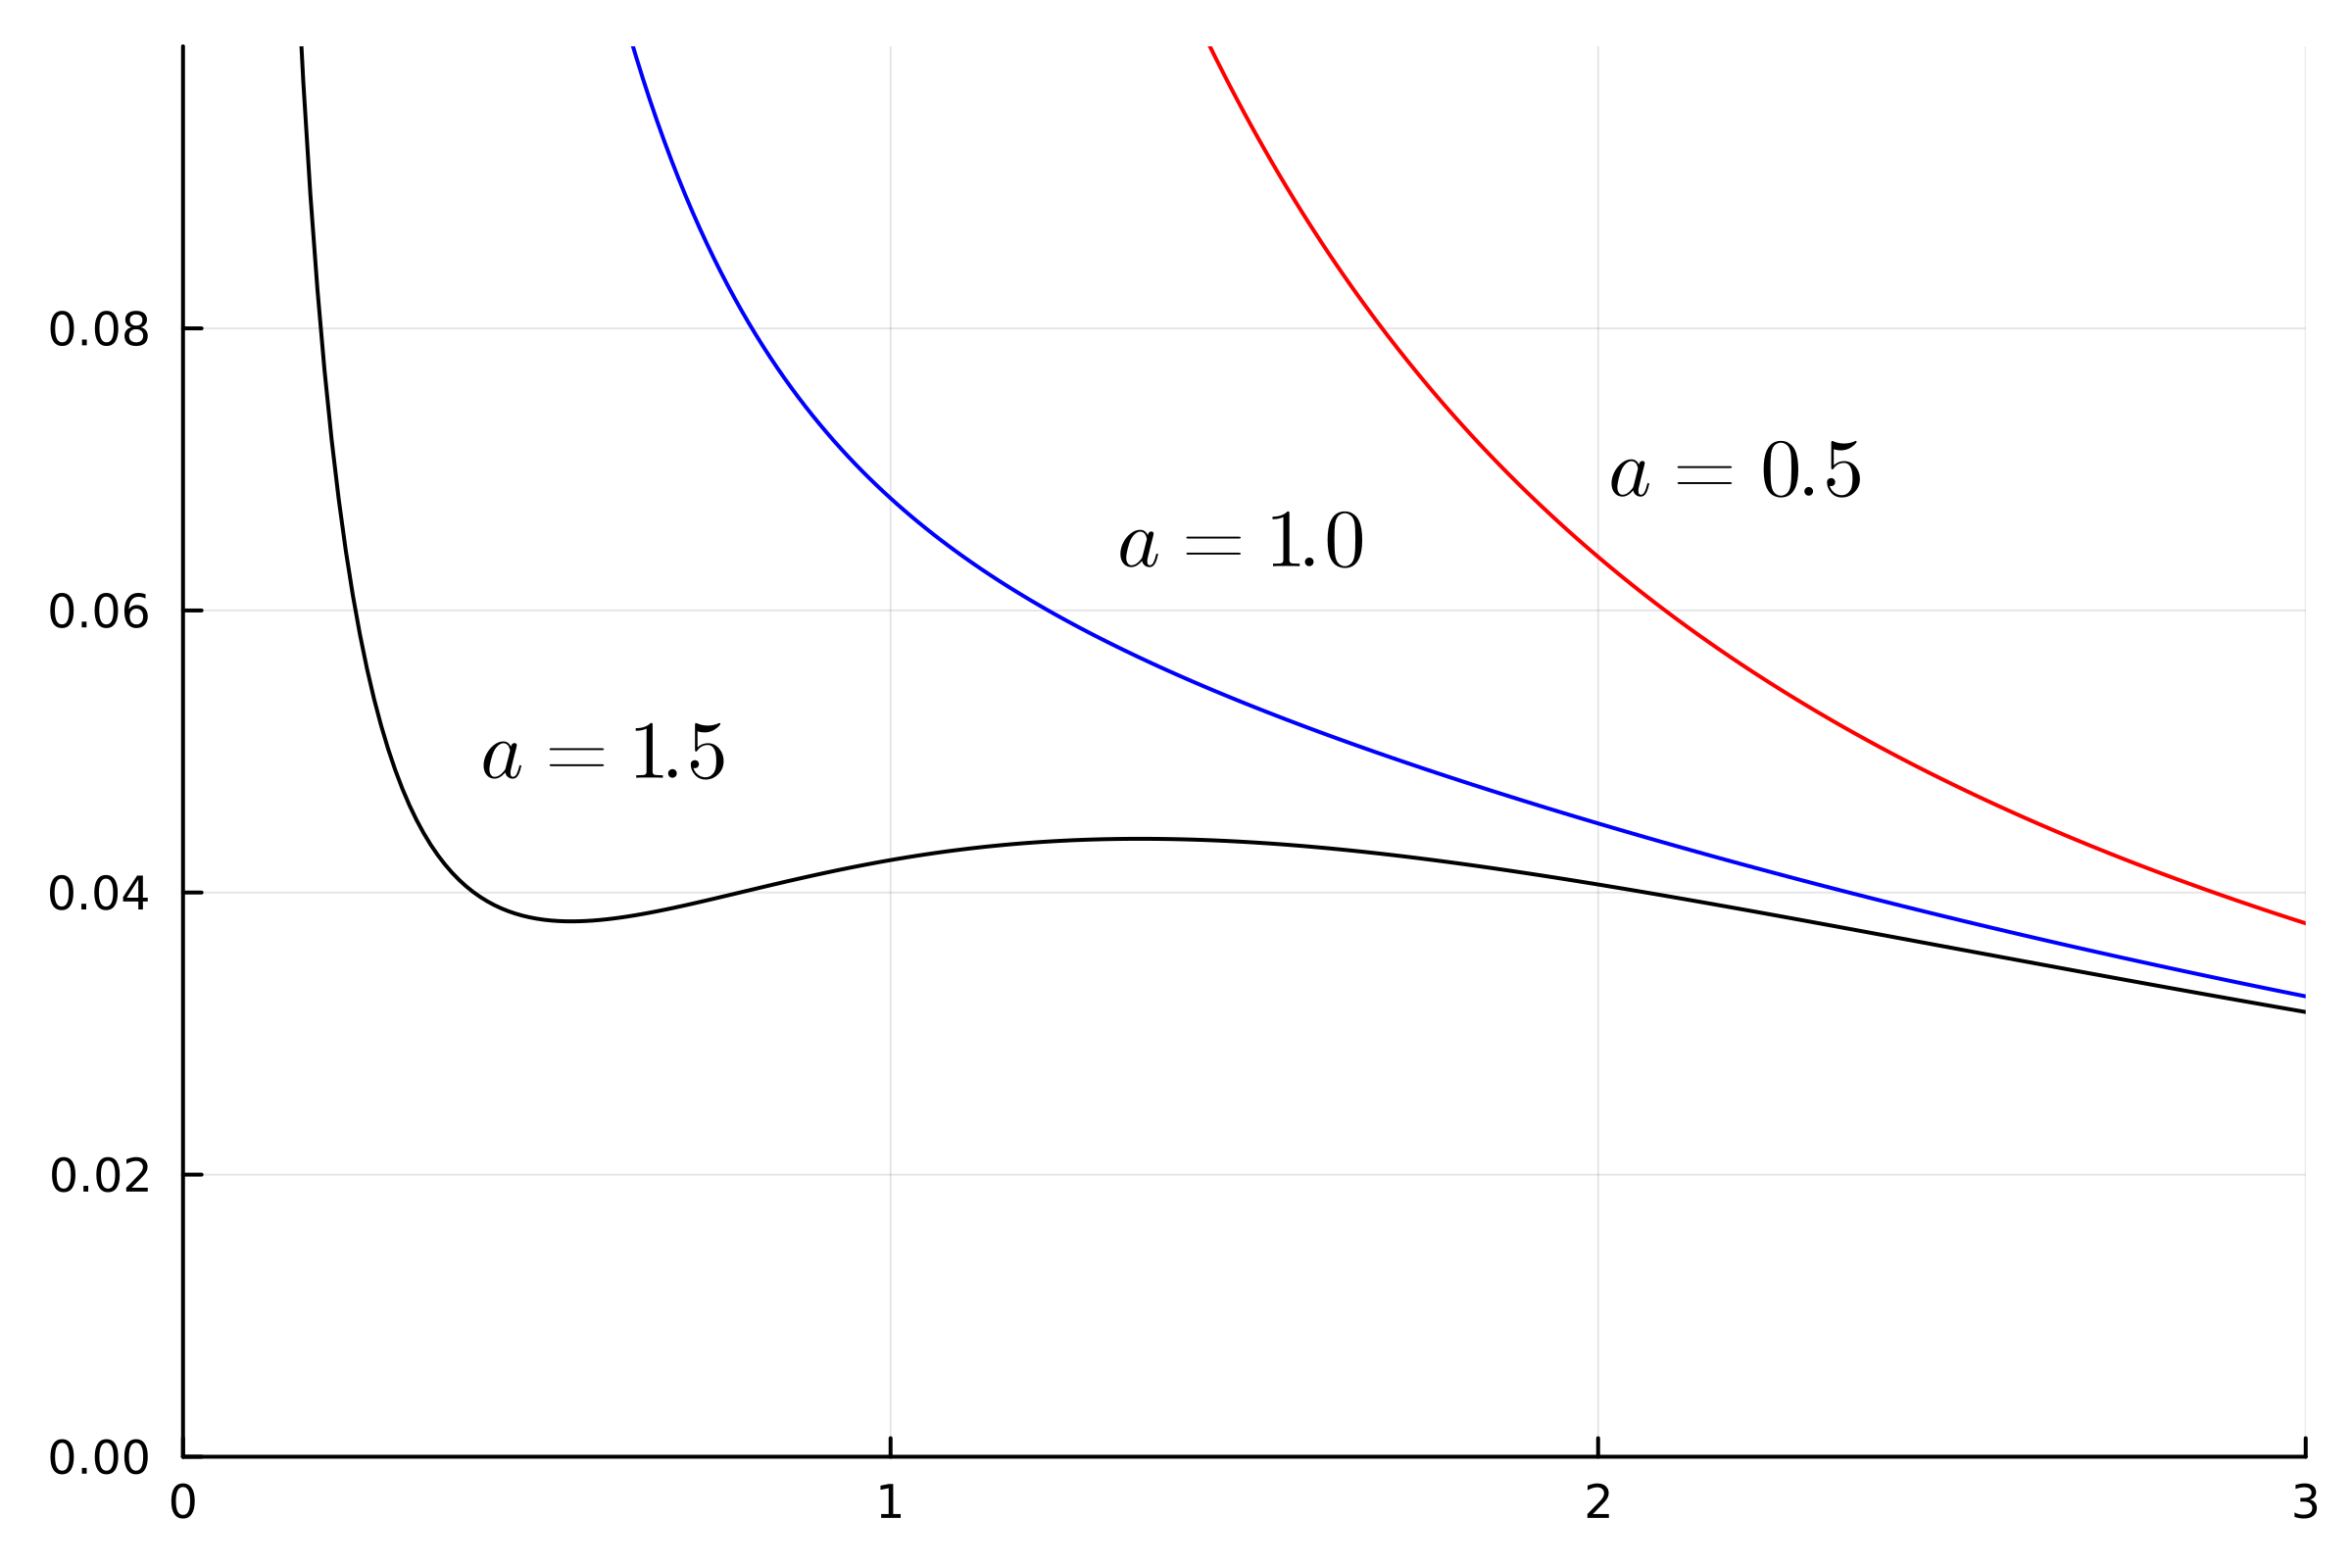
\includegraphics[width=0.5\columnwidth]{./images/buch/v-eff.png}
    \caption{並行移動}
    \label{}
\end{figure}

% リスト
\begin{enumerate}[(1)\,]
\item{}
\end{enumerate}

\end{document}